\documentclass[main.tex,fontsize=8pt,paper=a4,paper=portrait,DIV=calc,]{scrartcl}
% Document
\usepackage[T1]{fontenc}
\usepackage[dvipsnames]{xcolor}
\usepackage[nswissgerman,english]{babel}
\renewcommand{\familydefault}{\sfdefault}

% Format
\usepackage[top=5mm,bottom=1mm,left=5mm,right=5mm]{geometry}
%\setlength{\headheight}{\baselineskip}
%\setlength{\headsep}{0mm}

%\usepackage{scrlayer-scrpage}
%\clearpairofpagestyles
%\chead{{\bfseries\TITLE, \AUTHOR, \pagename~\thepage}}

%\addtokomafont{pagehead}{\upshape}

\usepackage{multicol}
\setlength{\columnsep}{2mm}
\setlength{\columnseprule}{0.1pt}

% Math
\usepackage{amsmath}
\usepackage{amssymb}
\usepackage{amsfonts}

% Code
\usepackage{fancyvrb, etoolbox, listings, xcolor}
%\usemintedstyle{bw}

%\newminted[shell]{bash}{
%fontsize=\footnotesize,
%fontfamily=tt,
%breaklines=true,
%frame=single,
%framerule=0.1pt,
%framesep=2mm,
%tabsize=2
%}
%\newminted{css}{
%breaklines=true,
%tabsize=4,
%autogobble=true,
%escapeinside=||,
%stripall=true,
%stripnl=true,
%}

    \definecolor{lightgray}{rgb}{0.95, 0.95, 0.95}
    \definecolor{darkgray}{rgb}{0.4, 0.4, 0.4}
    \definecolor{purple}{rgb}{0.65, 0.12, 0.82}
    \definecolor{ocherCode}{rgb}{1, 0.5, 0} % #FF7F00 -> rgb(239, 169, 0)
    \definecolor{blueCode}{rgb}{0, 0, 0.93} % #0000EE -> rgb(0, 0, 238)
    \definecolor{greenCode}{rgb}{0, 0.6, 0} % #009900 -> rgb(0, 153, 0)
    \definecolor{teal}{rgb}{0.0, 0.5, 0.5}

\lstdefinestyle{code}{
    identifierstyle=\color{black},
    keywordstyle=\color{blue}\bfseries\small,
    ndkeywordstyle=\color{greenCode}\bfseries\small,
    stringstyle=\color{ocherCode}\ttfamily\small,
    commentstyle=\color{teal}\ttfamily\textit\small,
    basicstyle=\ttfamily\small,
    breakatwhitespace=false,         
    breaklines=true,                 
    captionpos=b,                    
    keepspaces=true,                 
    showspaces=false,                
    showstringspaces=false,
    showtabs=false,                  
    tabsize=2,
    belowskip=-5pt
}



% Images
\usepackage{graphicx}
\newcommand{\pic}{\includegraphics[scale=0.3]}
\graphicspath{{Screenshots/}{../Screenshots}}
\makeatletter
\def\pictext#1#2{%
    \@ifnextchar[{%
    \pictext@iiiii{#1}{#2}%
    }{%
      \pictext@iiiii{#1}{#2}[0.5,0.4,0.3]% Default is 5
    }%
}
\def\pictext@iiiii#1#2[#3,#4,#5]{\begin{minipage}{#3\textwidth}\includegraphics[scale=#4]{#1}\end{minipage}\begin{minipage}{#5\textwidth}#2\end{minipage}}
\def\minipg#1#2{%
    \@ifnextchar[{%
    \minipg@iiii{#1}{#2}%
    }{%
      \minipg@iiii{#1}{#2}[0.3,0.6]% Default is 5
    }%
}
\def\minipg@iiii#1#2[#3,#4]{\vspace{0.8mm}\begin{minipage}{#3\textwidth}#1\end{minipage}\begin{minipage}{#4\textwidth}#2\end{minipage}{\vspace{0.8mm}}}
\makeatother

%\newenvironment{minty}[2]% environment name
%{% begin code
%  \begin{minipage}{#1}
%  \begin{minted}{#2}
%}%
%{% end code
%  \end{minted}
%  \end{minipage}
%  \end{minty}\ignorespacesafterend
%} 

% Smaller Lists
\usepackage{enumitem}
\setlist[itemize,enumerate]{leftmargin=3mm, labelindent=0mm, labelwidth=1mm, labelsep=1mm, nosep}
\setlist[description]{leftmargin=0mm, nosep}
\setlength{\parindent}{0cm}

% Smaller Titles
\usepackage[explicit]{titlesec}

%% Color Boxes
\newcommand{\sectioncolor}[1]{\colorbox{black!60}{\parbox{0.989\linewidth}{\color{white}#1}}}
\newcommand{\subsectioncolor}[1]{\colorbox{black!50}{\parbox{0.989\linewidth}{\color{white}#1}}}
\newcommand{\subsubsectioncolor}[1]{\colorbox{black!40}{\parbox{0.989\linewidth}{\color{white}#1}}}
\newcommand{\paragraphcolor}[1]{\colorbox{black!30}{\parbox{0.989\linewidth}{\color{white}#1}}}
\newcommand{\subparagraphcolor}[1]{\colorbox{black!20}{\parbox{0.989\linewidth}{\color{white}#1}}}

%% Title Format
\titleformat{\section}{\vspace{0.5mm}\bfseries}{}{0mm}{\sectioncolor{\thesection~#1}}[{\vspace{0.5mm}}]
\titleformat{\subsection}{\vspace{0.5mm}\bfseries}{}{0mm}{\subsectioncolor{\thesubsection~#1}}[{\vspace{0.5mm}}]
\titleformat{\subsubsection}{\vspace{0.5mm}\bfseries}{}{0mm}{\subsubsectioncolor{\thesubsubsection~#1}}[{\vspace{0.5mm}}]
\titleformat{\paragraph}{\vspace{0.5mm}\bfseries}{}{0mm}{\paragraphcolor{\theparagraph~#1}}[{\vspace{0.5mm}}]
\titleformat{\subparagraph}{\vspace{0.5mm}\bfseries}{}{0mm}{\subparagraphcolor{\thesubparagraph~#1}}[{\vspace{0.5mm}}]

%% Title Spacing
\titlespacing{\section}{0mm}{0mm}{0mm}
\titlespacing{\subsection}{0mm}{0mm}{0mm}
\titlespacing{\subsubsection}{0mm}{0mm}{0mm}
\titlespacing{\paragraph}{0mm}{0mm}{0mm}
\titlespacing{\subparagraph}{0mm}{0mm}{0mm}

%% format cells
\usepackage[document]{ragged2e}
\usepackage{array, makecell}
\renewcommand{\arraystretch}{2}
\newcommand{\mc}{\makecell[{{m{1\linewidth}}}]}



\lstset{
    language=[Sharp]C,
    style=code,
}
%%%%%

\begin{document}
\begin{table}[!ht]
\begin{tabular}{|m{0.2\linewidth}|m{0.755\linewidth}|}
\hline
The idea of 2d graphics & \vspace{2mm} \pic{2022-09-21-03:34:05.png} \\
\hline
2D projection & \parbox{0pt} Camera(\(e_{x},e_{y}\)) | Point(x,y) | c(x,y) = Transformed view | Equation: \( y = \dfrac{\Delta y}{\Delta z}z + c \) \,\,\,\ \raisebox{-.5\height}{\pic{2022-09-21-03:39:39.png}} \\
\hline
3D Model projection to 2D & \minipg{Camera(\( e_{x} , e_{y} , e_{z} \) | Point(x,y,z) \newline c(x,y,z) = transformed view \newline Equation:(\(c_{y}=\dfrac{e_{y}z-e_{z}y}{z-e{z}}\)) \newline Note this transformation must be done for ALL points!} {\pic{2022-09-21-04:28:04.png}}[0.4,0.6] \\
\hline
\textbf{How to draw a circle} & 
\begin{lstlisting}
float[] GetVertices(int sectors) {
    var vertices = new List<float>();
    float angle = 0;
    var deltaAngle = 2 * MathF.PI / sectors;
    //shift through all the sectors
    for (int sector = 0; sector < sectors; sector++) {
        //First we need to add the middle, which we can't do with the addpoint function,
        //since cosine and sine can't be 0 at the same time!!
        vertices.AddRange(new[] { 0f, 0f, 0f }); //point 0, aka middle
        AddCirclePoint(vertices, angle); //first triangle point 
        //The first triangle point will have a delta in only one axis
        angle += deltaAngle; // to get a delta in both x and y values we need a new angle.
        AddCirclePoint(vertices, angle); //third triangle point
    }
    return vertices.ToArray();
}

//This adds a single point with the cosine being x and y being sine.
//It can obviously be any other arrangement.
static void AddCirclePoint(List<float> vertices, float angle) {
    vertices.Add(MathF.Cos(angle)); // x
    vertices.Add(MathF.Sin(angle)); // y
    vertices.Add(0); //z
}

//The more sectors you add here the smoother the circle
//Fun fact, with 4 you get a rectangle, not a circle!
float[] vertices = GetVertices(4);
\end{lstlisting}\\
\hline
\end{tabular}
\section{Coordinate Models}
\begin{tabular}{|m{0,2\linewidth}|m{0.755\linewidth}|}
\hline
\textbf{local space} & 
\minipg{
The local space is the simple object inside an x,y,z system.\newline
Here x is to the right, y to the top, and z coming towards you.}
{\pic{2022-09-30-08:35:56.png}}[0.5,0.3]\\
\hline
\textbf{world space} & \minipg{
This is the actual representation inside the 3D world.\newline
It includes scaling and transformations.
}{\pic{2022-09-30-08:50:32.png}}[0.5,0.3]\\
\hline
\textbf{view space} & \minipg{
This view has it's z axis flipped. It now faces away from you.\newline
This is needed to properly handle the z axis that can't be seen in 2D\newline
but still needs to be there if you want the illusion of 3D.
}{\pic{2022-09-30-08:36:01.png}}[0.5,0.3]\\
\hline
\textbf{clip space} &
The clip space handles the above mentioned 3D illusion with a z-buffer.\\
\hline
\textbf{screen space} &
The actual view you will see on the screen, which obviously is 2D.\newline
It is the entire reason we are doing these shenanigans.\\
\hline
&\vspace{2mm} \pic{2022-09-30-08:37:05.png}\\
\hline
\end{tabular}
\end{table}
\pagebreak
\begin{table}[!ht]
\section{Transformations}
\begin{tabular}{|m{0,2\linewidth}|m{0.755\linewidth}|}
\hline
\textbf{\emph{Translation}}\newline 
\textcolor{teal}{\emph{This is not linear!}}
& \minipg{
A simple move of positions to another with a vector.\newline
\(\vec{a} + (x,y,z)\)(Point)
}{\pic{2022-09-30-09:31:39.png}}[0.5,0.4]\\
\hline
\textbf{\emph{Scaling}}\newline
\textcolor{teal}{\emph{This is always linear!}}
& \minipg{
A multiplication with a vector.\newline
\(s * \vec{a} = \vec{b}\)\newline
\textbf{Homogenous scaling}\newline
The homogenous scaling is simply 2D scaling with the z axis always being 1...\newline
\( \begin{bmatrix} a_1 \\ a_2 \\ 1 \end{bmatrix}  * \begin{bmatrix} x_{1} \, x_{12} \\ x_{21} \, x_{22} \\ 1 \end{bmatrix} \) 
}{\pic{2022-09-30-09:31:45.png}}[0.5,0.4]\\
\hline
\textbf{\emph{Rotation}} \newline
\textcolor{teal}{\emph{This is always linear!}}
& \minipg{
a rotation based on an angle that will be calculated\newline
based on cosine and sine. This will be applied to the x and y values.\newline
\pic{2022-09-30-09:32:13.png}
}{\pic{2022-09-30-09:32:04.png}}[0.5,0.4]\\
\hline
\end{tabular}
\section{Vectors}
\textbf{Notation} \( \vec{A} = \begin{bmatrix}x_{1} \\ x_{2} \end{bmatrix} \) OR \(\vec{A} = (x1 | x2)\)
\,   \,As you have learned in vocational school, use the first for vectors, the second for points.\\
\pictext{2022-09-23-10:41:26.png}
{A vector is nothing but a projection in the X,Y,Z planes \\ 
It has both a direction and a value\\
This value is usually modified by a scalar aka a factor. Then the vector can be something more universal \\
We call this universal vector a unit vector. A directional vector with the value 1.}[0.6,0.35,0.3]\\
\pictext{2022-09-23-10:41:32.png}{}[0.6,0.35,0.3]\\
\pictext{2022-09-23-10:41:37.png}{If the direction and the value is the same, then there is nothing that differentiates this vector from another.}[0.6,0.35,0.3]\\
\pictext{2022-09-23-10:41:44.png}{A vector is identical if both the value and the direction is the same.}[0.6,0.35,0.3]\\
\pictext{2022-09-23-10:41:48.png}{Similar, if the value is identical but the direction is negated, then you have the inverse vector.}[0.6,0.35,0.3]\\
\pictext{2022-09-23-10:41:53.png}{simple vector math}[0.6,0.35,0.3]\\
\subsection{Dotproduct}
\Large{\textbf{\textcolor{red}{\( \vec{a} * \vec{b} = |\vec{a}| * |\vec{b}| * sin(\alpha) * n \)}}}\newline
\normalsize This returns a scalar, aka a number that you can use.\newline
This will return 0 when used in a right angle as \(cos(90)\) is 0!\\
\subsection{Crossproduct}
\Large{\textbf{\textcolor{red}{\( \vec{a} \text{ x } \vec{b} = |\vec{a}| * |\vec{b}| * cos(\alpha) \)}}}\newline
\normalsize This is usually used to get the unit vector of the resulting vector.\newline
\(\alpha\) is the angle between the vector \(\vec{a}\) and \(\vec{b}\)\newline
\emph{\textcolor{teal}{For more information and proof, check the dedicated vector Document from vocational school.}}\\
\end{table}
\pagebreak
\begin{table}[!ht]
\begin{tabular}{|m{0.1\linewidth}|m{0.855\linewidth}|}
\hline
\textbf{Multiplication of vectors}
&
\textbf{Multiplication of vectors is not communitative!}\newline
\( \vec{AB} = \begin{bmatrix}\textcolor{blue}{x_{11} \, x_{12} \, x_{13}} \\ x_{21} \, x_{22} \, x_{23} \end{bmatrix} *
\begin{bmatrix} \textcolor{green}{y_{11}} \, y_{12} \\ \textcolor{green}{y_{21}} \, y_{22} \\ 
\textcolor{green}{y_{31}} \, y_{32}\end{bmatrix} =
\begin{bmatrix} \textcolor{red}{x_{11} * y_{11} + x_{12} * y_{21} + x_{13} * y_{31}} \,\,\, x_{11} * y_{12} + x_{12} * y_{22} + x_{13} * y_{32} \\
x_{21} * y_{11} + x_{22} * y_{21} + x_{23} * y_{31} \,\,\, x_{21} * y_{12} + x_{22} * y_{22} + x_{23} * y_{32}\end{bmatrix} =
\begin{bmatrix} \textcolor{red}{c_{11}} \, c_{12} \\ c_{21} \, c_{22} \end{bmatrix}\)\newline
\(\vec{BA} = \begin{bmatrix} \textcolor{blue}{x_{11} \, x_{12}} \\ x_{21} \, x_{22} \\ x_{31} \, x_{32} \end{bmatrix}
* \begin{bmatrix}\textcolor{green}{y_{11}} \, y_{12} \, y_{13} \\ \textcolor{green}{y_{21}} \, y_{22} \, y_{23} \end{bmatrix} =
\begin{bmatrix}\textcolor{red}{x_{11} * y_{11} + x_{12} * y_{21}} \,\,\, x_{21} * y_{11} + x_{22} * y_{21} \,\,\,
  x_{31} * y_{11} + x_{32} * y_{21} \\ x_{11} * y_{12} + x_{12} * y_{22} \,\,\, x_{21} * y_{12} + x_{22} * y_{22}\,\,\, x_{31} * y_{12} + x_{32} * y_{22} \\ x_{11} * y_{13} + x_{12} * y_{23} \,\,\, x_{21} * y_{13} + x_{22} * y_{23} \,\,\, x_{31} * y_{13} + x_{32} * y_{23}
\end{bmatrix} =
\begin{bmatrix} \textcolor{red}{c_{11}} \, c_{12} \, c_{13} \\ c_{21} \, c_{22} \, c_{23} \\ c_{31} \, c_{32} \, c_{33} \end{bmatrix}\)\newline
\textbf{\textcolor{red}{!! each row * each column !!}}\newline
\textbf{This also means that the row of the first matrix needs to be as long as the column of the second matrix!}\\
\hline
  \textbf{Determinant of a 2x2 matrix} &
For 2x2 matrices we can apply a simple trick to get the determinant.\newline
\textcolor{teal}{Note that this \textbf{only works for 2x2 matrices}}\newline
\( \vec{A} = \begin{bmatrix} a \, b \\ c \, d \end{bmatrix} \)\newline
Determinant >> \(det(a) = a * d - b * c  = ad - bc\)\\
\hline 
  \textbf{Determinant of any square matrix} &
  \textcolor{red}{\textbf{\underline{!! This is only possible for square matrices !!}}}\newline
  \pic{2022-10-05-04:07:24.png} \pic{2022-10-05-04:09:33.png}\newline
  \textcolor{teal}{We take the first character, then exclude the row and column of that character and instead multiply the character with the matrix of the remaining characters.\newline
  Continue this until you have 2x2 matrices which you can instantly solve.\newline} 
  \textbf{\textcolor{red}{Note: the determinants are added together in a fluctuating way. \newline
  The first is subtracted, then the next added, next subtracted again and so forth.}}\\
\hline
\textbf{linear dependency} & \minipg{
A vector is linearly dependent to another if the addition of 2 vectors, each multiplied by a scalar, can be equal to the NULL vector.\newline \textcolor{teal}{The only restriction is that at least 1 scalar needs to be \textbf{non-zero}}} 
{\pic{2022-10-05-04:19:15.png}\pic{2022-10-05-04:22:25.png}}[0.45,0.5]\newline
In this case the vectors are indeed linearly independent as the only solution of \(x * \vec{A} + y * \vec{B} = 0\) was \(x=0 \,\,\, y=0\).\newline
\, \newline
\textbf{Second method: Determinant}\newline
You can merge the two vectors and then take the determinant to check for linear dependency. \newline
Make sure the resulting vector is a square as this method won't work otherwise.\newline
\begin{itemize}
  \item \textcolor{teal}{If the \textbf{determinant is 0} then the vectors are \textbf{linearly dependent}}
  \item \textcolor{teal}{If the \textbf{determinant is not 0} then the vectors are \textbf{linearly independent}}
\end{itemize}
\, \newline
\textbf{Third method:}\newline
The third method requires the \textcolor{teal}{GAUSS algorithm}.\newline
With this we can merge any number of vectors into a matrix and then add/subtract lines from them.\newline
It is the same thing you do when calculating the result of a linear set of equations.\newline
In other words simply add or subtract rows to or from other rows with any scalar applied to it.\newline
\pic{2022-10-05-04:36:11.png} \pic{2022-10-05-04:36:25.png}\newline
\textcolor{teal}{If the result gets a unit matrix, then the vectors are linearly independent,\newline
as further calulation would result in all scalars being 0 to get to the NULL vector!\newline
If the result does not match the unit matrix, aka the diagonal line is not made of 1's, \newline
the vectors are linearly dependent.}\\
\hline
\textbf{Inverse of a 2x2 Matrix} & \minipg{
The inverse of a 2x2 matrix is easy just like the determinant.\newline
Simply swap a with d, and invert both b and c.\newline
Then multiply this with the inverse of the determinant of the original matrix.}
{\pic{2022-10-05-05:07:54.png}}[0.4,0.5]
\\
\hline
\textcolor{teal}{Linearity} &
Linearity means that something can be done in reverse.\newline
For example a function is linear if the following is true:\newline
\large \textcolor{teal}{\( f(\vec{a} + \vec{b}) = f(\vec{a}) + f(\vec{b}) \) \newline
OR\newline 
\( f(a * \vec{a}) = a* f(\vec{a}) \)}
\normalsize
\\
\hline
\end{tabular}
\end{table}
\pagebreak
\begin{table}[!ht]
\begin{tabular}{|m{0.1\linewidth}|m{0.855\linewidth}|}
\hline
\textbf{Inverse of any matrix} & 
\minipg{
In the first step we calculate all the different determinants into a new matrix.\newline
In other words, for each element in the matrix we calculate the determinant of the matrix not in the row or column of that element, just like determinants before!.
}
{\pic{2022-10-05-05:07:54.png}}[0.4,0.5] \newline
\, \newline
\minipg{
Here we invert some of the elements in the matrix with a checkerboard of + an -.\newline
+ - +\newline
- + -\newline
+ - +
}
{\pic{2022-10-05-05:05:57.png}}[0.4,0.5] \newline
\, \newline
\minipg{
Now we swap the right top side with the bottom left side.\newline
The diagonal line in the middle will stay untouched.
}
{\pic{2022-10-05-05:06:33.png}}[0.4,0.5] \newline
\, \newline
\minipg{
Now divide your resulting matrix with the determinant of the original matrix. haha fun....
}
{\pic{2022-10-05-05:07:21.png}}[0.4,0.5] \\
\hline
Inverse of Orthogonal Matrix & 
\textcolor{red}{\textbf{If a matrix is orthogonal, meaning that all 3 vectors are 90degrees apart from each other,\newline
then you can simply use the transpose of said matrix for the inverse!}}\\
\hline
Transpose of Matrix & 
\huge \(\vec{A} = \begin{bmatrix} a & b & c \\ d & e & f \end{bmatrix} \) \,\,\,\,\,\,\, \(\vec{A}^T = \begin{bmatrix} a & d \\ b & e \\ c & f\end{bmatrix} \)\newline
\large \textcolor{orange}{Also:}\newline
\huge \( \vec{v}^T * \vec{A}^T = (\vec{Av})^T \)
\normalsize \\
\hline
\end{tabular}
\end{table}
\begin{table}[ht!]
\section{Planes in Viewport}
\begin{tabular}{|m{0.2\linewidth}|m{0.755\linewidth}|}
\hline
Near and Far clip plane\newline
Fov &
\minipg{
\begin{itemize}
  \item \textbf{\textcolor{orange}{Far Clip Plane}}
    This is the maximum distance (z axis) on which an object is still rendered
  \item \textbf{\textcolor{orange}{Near Plane}}
    This is the smallest distance (z axis) on which an object is still rendered
  \item \textbf{\textcolor{orange}{FOV}}
    This is the angle at which we look at the world\newline
    \textcolor{teal}{\emph{The higher this is, the more we see, but everything appears smaller!}}
  \vspace{-3mm}
\end{itemize}
}
{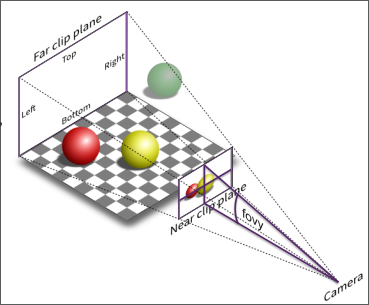
\includegraphics[scale=0.4]{2022-10-12-03:18:06.png}}[0.4,0.5]\\
\hline
Colors & 
\minipg{
Colors are also represented as a vector:\newline
\textcolor{red}{\( \vec{red} = \begin{bmatrix} 1 & 0 & 0 \end{bmatrix} \)}\newline
\textcolor{green}{\( \vec{green} = \begin{bmatrix} 0 & 1 & 0 \end{bmatrix} \)}\newline
\textcolor{blue}{\( \vec{blue} = \begin{bmatrix} 0 & 0 & 1 \end{bmatrix} \)}
}
{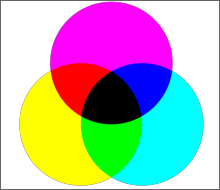
\includegraphics[scale=0.4]{2022-10-12-03:50:36.png}}\\
\hline
Colors from multiple sources & 
If you have more than 1 light source for a color, then these result in an additive colormix.\newline
\, \newline
 \textcolor{orange}{\huge \( c = 1 - ( 1 - c_{L1})^T * (1 - C_{L2}) \)}\newline
\, \newline
\normalsize \textcolor{teal}{Here the light is equal to 1 minus the transpose of (1 - light source 1) * (1 - light source 2) }\\
\hline
GPU Pipeline & \minipg{
The pipeline consists of:\newline
\begin{itemize}
  \item \textcolor{orange}{Vertex Processor}\newline 
    Handles raw vertices and primitives\newline
    Defines how the structure will look\newline
    Transforms points into clip-space\newline
    \textcolor{teal}{-- Programmable --}
  \item \textcolor{orange}{Rasterizer} \newline
    Transformed Vertices and Primivtes\newline
    fills the structure
  \item \textcolor{orange}{Fragment Processor} \newline
    Fragments\newline
    Defines color and things such as anti-aliasing\newline
    \textcolor{teal}{-- Programmable --}
  \item \textcolor{orange}{Output Merging} \newline
    Processed Fragments\newline
    Handles output merging
\end{itemize}
}{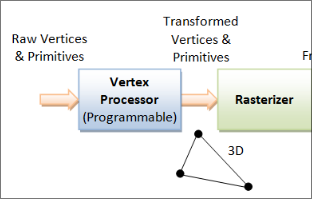
\includegraphics[scale=0.45]{2022-10-12-04:02:08.png}\newline
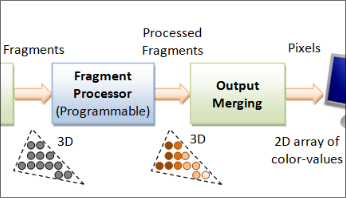
\includegraphics[scale=0.45]{2022-10-12-04:02:16.png}}[0.4,0.4]\\
\hline
  Double Buffering & 
  \textcolor{orange}{Instead of updating the frame that we show on the screen directly, we update a buffer first in order to avoid artifacts on the screen.\newline
  This buffer is then synchronized every x frames.\newline}\\
\hline
  Normalized Device Coordinates & 
  \textcolor{orange}{These are coordinates between 0 and 1. Graphics API \textbf{require} these.}\\
\hline
  Normals for Lighting & 
  \textcolor{orange}{Lighting is usually done by checking the normalvector of the surface, in other words by checking the orientation of the surface, is it looking towards the light or away? And with what angle?\newline
  All this can be done with the normal.}\newline
  A Normal can be obtained in 2 ways:\newline
  \begin{itemize}
    \item \textcolor{teal}{Storing it within the model}
    \item \textcolor{teal}{Calculating it on the fly}
    \vspace{-3mm}
  \end{itemize}\\
\hline
  Diffusion & \minipg{
  \textcolor{orange}{Diffusion is the reflection of light based on the angle of the surface.\newline
  This should only be done with matte surfaces, as glossy would reflect differently.}
  }
  {\pic{2022-10-19-02:15:57.png}}[0.5,0.4]\\
\hline 
  Specular Lighting & \minipg{
  \textcolor{orange}{Reflection of light on a glossy surface.\newline
  Instead of diffusing the light, a glossy surface simply returns the light at another angle, \newline
with likely a bit less power!}}
  {\pic{2022-10-19-02:20:34.png}}[0.5,0.4]\\
\hline 
Phong Shading & \minipg{
\textcolor{orange}{\textbf{A combination of ambient, diffusion and specular lighting}}\newline
\textcolor{red}{After 90 degrees, there is no more reflection! \newline 
Unless the surface is not smooth -> some parts don't have above 90 degree angle}}
{\pic{2022-10-19-02:44:07.png}}[0.5,0.4] \\
\hline
Blinn-Phong Shading & \minipg{
\textcolor{orange}{Solves the issue from Phong shading with the 90 degree angle, by using a halfway vector.}}
{\pic{2022-10-19-02:44:13.png}}[0.5,0.4]\\
\hline 
\end{tabular}
\end{table}
\pagebreak
\begin{table}[ht!]
\section{Meshes}
\begin{tabular}{|m{0.2\linewidth}|m{0.755\linewidth}|}
\hline
Polygon Mesh & \minipg{
\textcolor{green}{Pro:}\newline
\begin{itemize}
  \item \textcolor{teal}{any geometry possible}
  \item \textcolor{teal}{any accuracy possible}
  \item \textcolor{teal}{flexible: direct GPU support, most used}
  \item \textcolor{teal}{relatively easy and performant computing}\newline
    Transformations and overlapping with straight lines
\end{itemize}
}
{
\textcolor{red}{Con:}\newline
\begin{itemize}
  \item \textcolor{teal}{fixed accuracy (after you chose one)}
  \item \textcolor{teal}{relatively high memory usage}
  \item \textcolor{teal}{increasing computing time with many primitives}\newline 
  \, \newline
  \, \newline
  \, \newline
  \vspace{-3mm}
\end{itemize}
}[0.4,0.4]\\
\hline
Triangulation & 
\textcolor{orange}{Triangulation means the creation of triangles from dots to form a shape}\newline
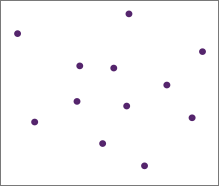
\includegraphics[scale=0.45]{2022-10-19-03:19:55.png}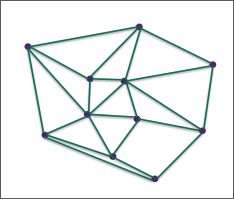
\includegraphics[scale=0.45]{2022-10-19-03:19:58.png}\\
\hline
Sweep Strategy \newline in Triangulation & 
\vspace{2mm}
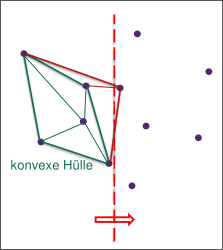
\includegraphics[scale=0.45]{2022-10-19-03:21:54.png}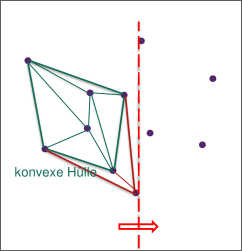
\includegraphics[scale=0.45]{2022-10-19-03:22:00.png}\newline
\textcolor{orange}{The idea is to always move from left to right and connect the closest 3 triangles,\newline
\textbf{where no edge crosses another!}\newline
This means that we will get at least 3 lines on each point!}\\
\hline
Insert Strategy \newline in Triangulation & 
\vspace{2mm}
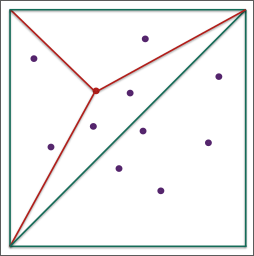
\includegraphics[scale=0.45]{2022-10-19-03:28:11.png}\newline
\textcolor{orange}{1. We start with triangles around the points, these are here the green triangles.\newline
2. Then we choose a random point within one of these triangles.\newline
3. We go to each edge of the triangle from that point\newline
4. Remove unnecessary triangles ???????? WAT}\\
\hline
Delaunay Triangulation \newline Edge Flip &
\textcolor{orange}{Both the sweep strategy and the insert strategy have a problem, \newline
Inside of these triangles, there might be a shorter edge than the current chosen one, in this case, \newline
We would lose performance, this is why we use \textbf{edge flip}, this essentially means using the shorter,\newline
and therefore faster edge instead.}\newline
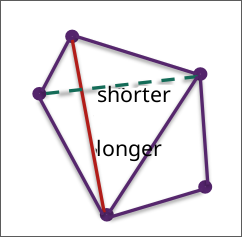
\includegraphics[scale=0.45]{2022-10-19-03:36:45.png}\\
\hline
Heat Maps & \minipg{
\textcolor{orange}{A simple projection of a function: }\newline
\huge \textcolor{teal}{\( p = f(x,y) \)}\newline
\huge \textcolor{teal}{\( p = f(x,y,z) \)}
\normalsize
}{
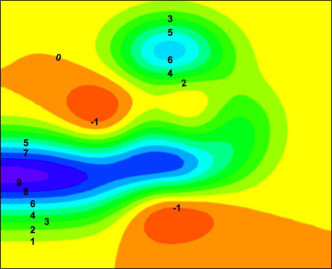
\includegraphics[scale=0.45]{2022-10-19-03:40:57.png}}[0.3,0.4]\\ 
\hline
\end{tabular}
\end{table}
\pagebreak
\begin{table}[ht!]
\begin{tabular}{|m{0.2\linewidth}|m{0.755\linewidth}|}
\hline
Interpolation & 
\begin{tabular}{m{0.3\linewidth}m{0.3\linewidth}m{0.3\linewidth}}
\textcolor{orange}{Polynomial Interpolation}\newline
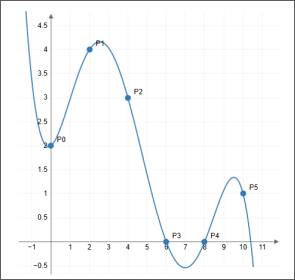
\includegraphics[scale=0.4]{2022-10-19-03:46:45.png}\newline
\textcolor{teal}{Polynomials of grade n can interpolate n+1 points}
&
\textcolor{orange}{Quadratic Interpolation -> Polynomial power 2}\newline
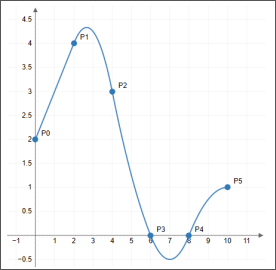
\includegraphics[scale=0.4]{2022-10-19-03:46:49.png}\newline
\textcolor{teal}{Since we can only interpolate 3 points here,\newline
We have to add rules -> see analysis 1 in order to make this work}
&
\textcolor{orange}{Cubic Interpolation -> Polynomial power 3}\newline
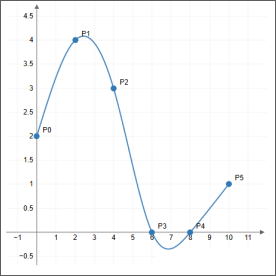
\includegraphics[scale=0.4]{2022-10-19-03:46:53.png}\newline
\textcolor{teal}{The same thing with power 3 -> just with less rules}
\\
\end{tabular}\\
\hline
NURBS & 
\textcolor{orange}{non-uniform rational B-Splines}\newline
This is used in things like CAD programs, they are essentially the points to interpolate,\newline
you use this to change the forms in these programs.\\
\hline
Lindenmayer & 
\textcolor{teal}{Lindenmayer is a strange system to draw graphics by using forward movement:\newline
for example f+f+f+ angle=90 means 3 times forward in positive and then doing a 90 degree turn.\newline
This is essentially what people do in highschool, lmao}\newline
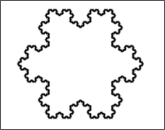
\includegraphics[scale=0.4]{2022-10-26-02:14:35.png}\\
\hline
Koch Snowflake & 
\textcolor{orange}{The idea here is that an infinite amount of added bends will create a finite area, but an infinite line.}\newline
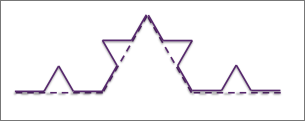
\includegraphics[scale=0.4]{2022-10-26-02:21:43.png}\newline
\textcolor{teal}{The triangles are the bends, the area is the are between the full and dashed line.}\\
\hline
Hilbert Curve & 
\textcolor{teal}{Essentially procedural filling of a figure:}\newline 
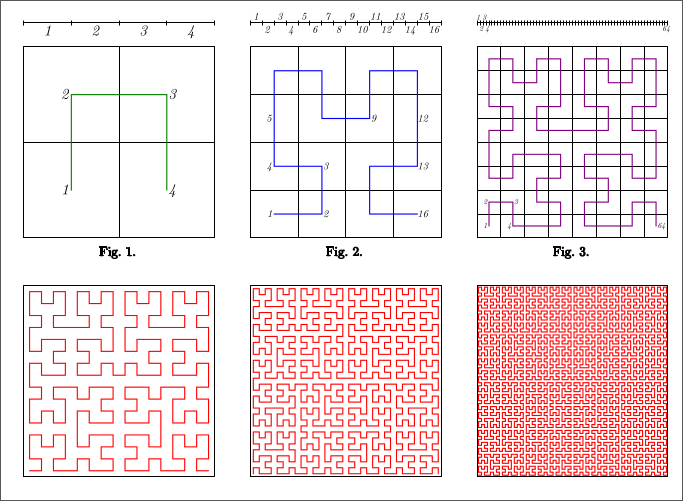
\includegraphics[scale=0.4]{2022-10-26-02:22:50.png}\\
\hline
Fractals & 
\textcolor{orange}{Fractals are the idea of recursively creating a 3D structure, usually a tree:}\newline
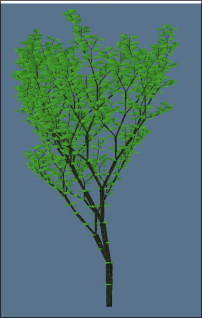
\includegraphics[scale=0.35]{2022-10-26-02:26:27.png}\newline
\textcolor{teal}{Usually these do not look as natural as this one, but this is of course the goal}\\
\hline
\end{tabular}
\end{table}
\pagebreak
\begin{table}[ht!]
\begin{tabular}{|m{0.2\linewidth}|m{0.755\linewidth}|}
\hline
Recursive flattening & 
\textcolor{orange}{This is nothing else other than the smoothing of a structure by recursively exchanging hard surfaces with smaller ones to make them look more smooth:}\newline
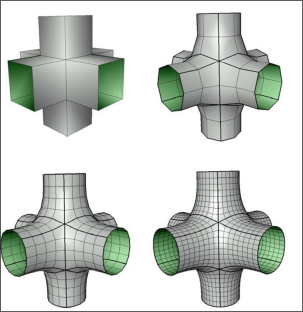
\includegraphics[scale=0.4]{2022-10-26-02:32:46.png}\newline
\textcolor{teal}{This is essentially similar to what you do with the sphere, where you can define how many vertices you want to build.}\newline
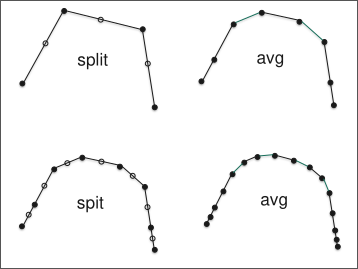
\includegraphics[scale=0.4]{2022-10-26-02:37:46.png}\newline
\textcolor{teal}{Here we split the splines in the middle of each line and create another point.}\\
\hline
\end{tabular}
\subsection{Terms in Meshes}
\begin{tabular}{|m{0.2\linewidth}|m{0.755\linewidth}|}
\hline
Terms &
\begin{itemize}
\item \textcolor{orange}{Valence: Count of incoming and outgoing edges}
\item \textcolor{orange}{Boundary: outer edges of polygon}
\item \textcolor{orange}{Completely regular: all nodes are regular}
\item \textcolor{orange}{Mostly regular: most nodes are regular}
\item \textcolor{orange}{irregular: rest}
\vspace{-3mm}
\end{itemize}\\
\hline 
Irregular and Regular Nodes & 
\textcolor{orange}{A node is regular if it has exactly 6 incoming/outgoing edges if the node is inside the polygon and exactly 4 incoming/outgoing edges if it is an edge node.}\newline
\textcolor{orange}{A node is irregular if it has 4 edges if inside and 3 if edgenode}\\
\hline
Model Repair & 
\textcolor{orange}{There are 2 main ways to repair a model: Area based algorithms and Volume based algorithms:}\newline
\minipg{
\textcolor{teal}{Area based:}\newline
\begin{itemize}
  \item \textcolor{green}{ Surface characteristics stay} 
  \item \textcolor{red}{ inferior detection and solving of errors } 
    \, \newline
    \, \newline
\end{itemize}
}{
\textcolor{teal}{Volume based:}\newline
\begin{itemize}
  \item \textcolor{green}{ Good detection and solving of errors} 
  \item \textcolor{red}{ often too detailed, with subpar triangulation quality\newline
    Therefore surface characteristics are lost} 
\end{itemize}
}[0.4,0.4]\\
\hline
Vertex Clustering & 
\textcolor{orange}{This is the gradual reduction of trianges, while keeping the shape of the mesh.}\newline
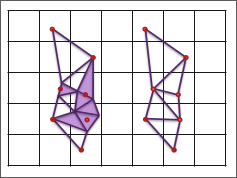
\includegraphics[scale=0.4]{2022-10-26-03:37:42.png}\newline
\textcolor{teal}{Each triangle that has 2 nodes in one square gets eliminated, based on how big, or how small these squares are the clustering leads to a worse approximation of the structure!}\\
\hline
\end{tabular}
\end{table}
\pagebreak
\begin{table}[ht!]
\section{Rasterization and Aliasing}
\begin{tabular}{|m{0.2\linewidth}|m{0.755\linewidth}|}
\hline
Rasterization & 
\textcolor{orange}{This is the projection of pixels in a triangle.}\newline
\textcolor{red}{\textbf{Here only the pixels are colorized -> shown, that have their center inside the triangle!}}\newline
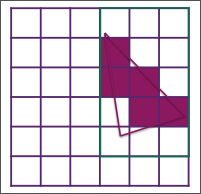
\includegraphics[scale=0.4]{2022-11-02-04:24:11.png}\\
\hline
Z-Buffer in Rasterization & 
\textcolor{orange}{In order to specify which object is closer to the camera, we can use the z buffer with different color values to represent this axis.}\newline
\, \newline
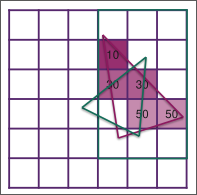
\includegraphics[scale=0.45]{2022-11-02-04:24:20.png}
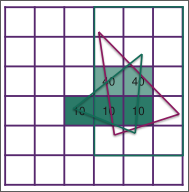
\includegraphics[scale=0.45]{2022-11-02-04:24:29.png}
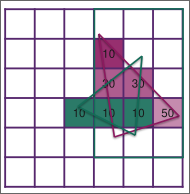
\includegraphics[scale=0.45]{2022-11-02-04:24:35.png}\\
\hline
\end{tabular}
\end{table}
\pagebreak
\begin{table}[ht!]
\begin{tabular}{|m{0.2\linewidth}|m{0.755\linewidth}|}
\hline
Z-Precision & 
\textcolor{orange}{Due to the loss of floating point precision, if you have things that are too close together, you can have so called \textbf{Z-Fighting}, this happens when the value is nearly identical, and it therefore might choose parts of one and parts of the other.}\newline
\textcolor{purple}{This essentially is flimering in games!}\\
\hline
Aliasing & 
\textcolor{orange}{Due to the fact that we ignore all pixels that are not withing the triangle, we will lose precision, which will often represent itself as the staircase like aliasing. This means that the projection will have very sharp and unnatural edges.}\\
\hline
Anti-Aliasing & 
\textcolor{orange}{This is the counter to the staircase problem that smoothes the edges.}\newline
\textcolor{pruple}{It essentially uses the same trick as the Z-Buffer to generate values that then have colorization based on the value:}\newline
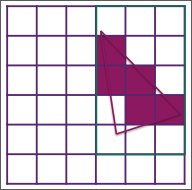
\includegraphics[scale=0.45]{2022-11-02-04:45:00.png} 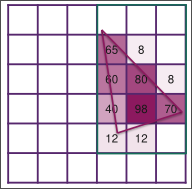
\includegraphics[scale=0.45]{2022-11-02-04:45:06.png}\\
\hline
Super-Sampling & 
\textcolor{purple}{This is essentially the little brother of anti aliasing, it calculates the same thing as the aliasing does with 4 points instead of one.\newline
Then it will pick the color strength based on how many points are inside the triangle, if none are inside the triangle, then it will not be colorized}\newline
\, \newline
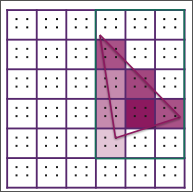
\includegraphics[scale=0.45]{2022-11-02-04:48:13.png}\\
\hline
Mipmaps & 
\textcolor{orange}{The super sampling method doesn't work for textures as it is only done once per pixel.\newline
Here we can solve this issue by creating multiple textures that will be applied when needed.\newline
In other words, the system will take another texture as soon as you are either too close or too far away form the polygon.}\newline
\, \newline
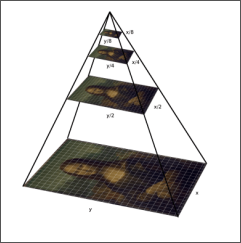
\includegraphics[scale=0.45]{2022-11-02-05:05:00.png}\\
\hline
\end{tabular}
\section{Reflections and Shadows}
\begin{tabular}{|m{0.2\linewidth}|m{0.755\linewidth}|}
\hline 
Reflection on surfaces & 
\textcolor{orange}{The idea is that you have a mirror and you want to show the reflection of that object in a mirror. Here you would create a virtual reflection camera that will project this object onto this surface.}\newline
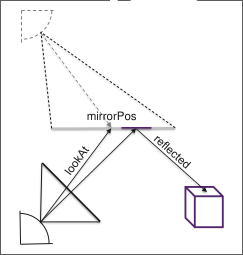
\includegraphics[scale=0.45]{2022-11-02-05:17:03.png}\\
\hline
Shadow Mapping & 
\textcolor{orange}{The idea is very simple, use the original light source as vector source and then project the object that should throw a shadow to the surface in question. \newline
Here instead of using the same colors, we only use the same depth, the color will be the shadow color!}\newline
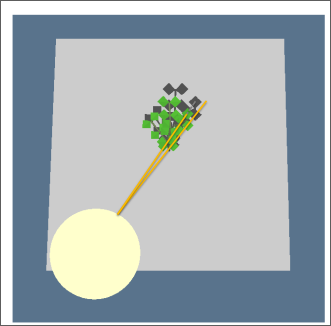
\includegraphics[scale=0.36]{2022-11-02-05:12:34.png}\\
\hline
\end{tabular}
\end{table}
\pagebreak
\begin{table}[ht!]
\begin{tabular}{|m{0.2\linewidth}|m{0.755\linewidth}|}
\hline 
Shadow Mapping example code &
\vspace{2mm}
\begin{lstlisting}
var lookingVector = position - _light.Position;
float sinFovy = height / lookingVector.Length;
float fovy = MathF.Asin(sinFovy);
var projection = Device.GetPerspectiveProjection(
  fovy, width / height, 0.1f, 100.0f);
var view = new CameraView(
  _light.Position,
  lookingVector.Normalized(),
  Device.World.Unit3Y);
  lightViewProjection = Device.GetViewMatrix(view) * projection;
var shadow = Device.TakeDepthPicture(
  Scene, size,
  _light.Ambient.GetColor4(1),
  _light.Position, view, projection);
\end{lstlisting}\\
\hline
General Reflections & 
\textcolor{orange}{General reflections are done by reflecting an object against a texture, this can of course als be an object:}\newline
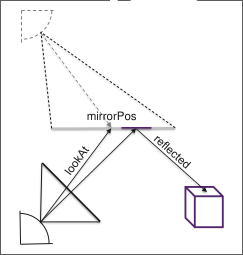
\includegraphics[scale=0.4]{2022-11-02-05:17:03.png}\\
\hline
Projection of different objects & 
\textcolor{orange}{You can project a texture for a different type of object to another by essentially cutting it into pieces. For example you might take a texture for a sphere and use it on a cube:}\newline
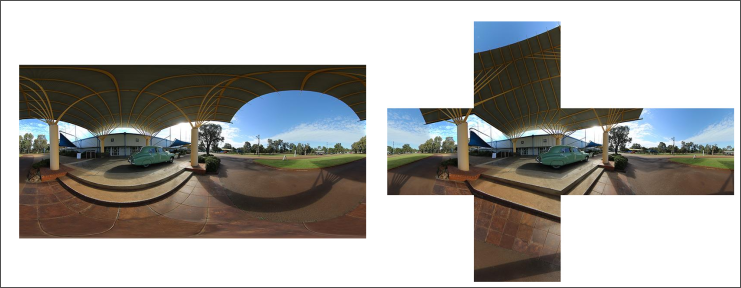
\includegraphics[scale=0.4]{2022-11-02-05:27:46.png}\\
\hline
Depth-Map&
\textcolor{orange}{This is simply a visualization of the Z-Buffer:}\newline
\textcolor{purple}{white = far away\newline
balck = close}\\
\hline
\end{tabular}
\end{table}
\pagebreak
\begin{table}[ht!]
\section{}
\begin{tabular}{|m{0.2\linewidth}|m{0.755\linewidth}|}
\hline

\hline
\end{tabular}
\end{table}
\pagebreak
\begin{table}[ht!]
\section{}
\begin{tabular}{|m{0.2\linewidth}|m{0.755\linewidth}|}
\hline

\hline
\end{tabular}
\end{table}
\end{document}

